\subsection {Exams, Exercise 2}

\lineparagraph {Exercise}

Construct a deterministic finite automaton that accepts thos words from $(0+1)*$ that contain subword $010$ exactly once. (For example $0100110$ is an element of the language, however $010010$ and $01010$ do not belong to it.)

\lineparagraph {Solution}

The first subtask to do is to construct a DFA that accepts words that contain the $010$ subword (without the other requirements):

\begin{center}
    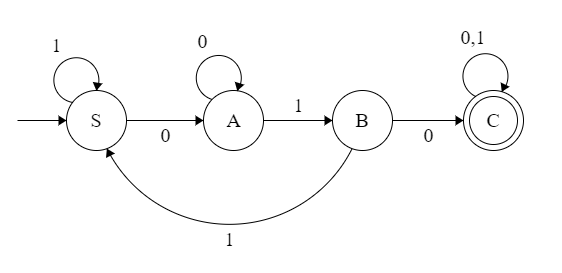
\includegraphics[width=\linewidth]{./exams/misc/02/step_1.png}
\end{center}

All of the states represent how long of a prefix we have received so far: S for no useful prefix, $A$ for the ''$0$'' being the last character we have read and possibly continuing with ''$10$'' after, $B$ for the $10$ word being the last two characters we have read and possibly continuing with ''$0$'' and finally C means we have read the entire word.

Whenever we receive one more matching character, we move upwards, while if we receive the other character we need to fail back some steps. In state $S$, if we get $1$'s we just stay in $S$, that is not useful, we need a $0$ to start. In state $A$, if we receive $0$'s, we can stay in $0$, since the last $0$ character is useful to us. In state $B$, if we receive a $1$, that ruins everything, we know that that means the last characters on the input were $011$, which has no useful parts to us, we fail back to $S$.

Notice additionally, that this automaton reaches the state $C$ the \textbf{first time} it finds the $010$ on the input.

This means that if we start trying to find another $010$ there, in a similar manner, we can detect a second $010$. We cannot start in $C$, however, $C$ should already mean the $0$ was received, so we kind of copy and paste this DFA onto itself, the next copy having $S' = B and A' = C$, like so:

(And remove the looping on the original $C$.)

\begin{center}
    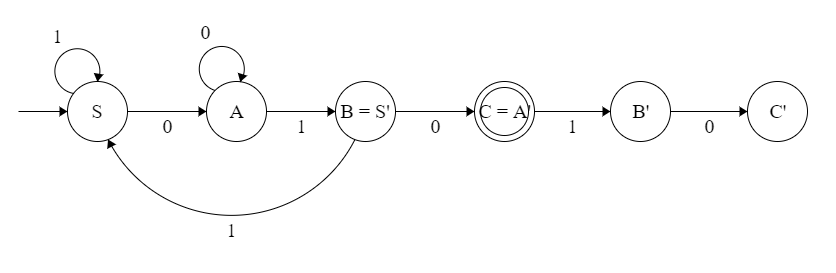
\includegraphics[width=\linewidth]{./exams/misc/02/step_2.png}
\end{center}

I have added the forward pointing transitions, and now we need to be really careful about the backward pointing ones:

There is a loop of $1$'s in state $S$, this is waiting for the computation to start. We cannot add this to $B=S'$, because there is already a $1$ exiting from it. However, we need a similar function in the second part of the automata, something that we can go back to when nothing matches, and we can wait there until we are reading $1$'s. So for this, we introduce a new state:

\begin{center}
    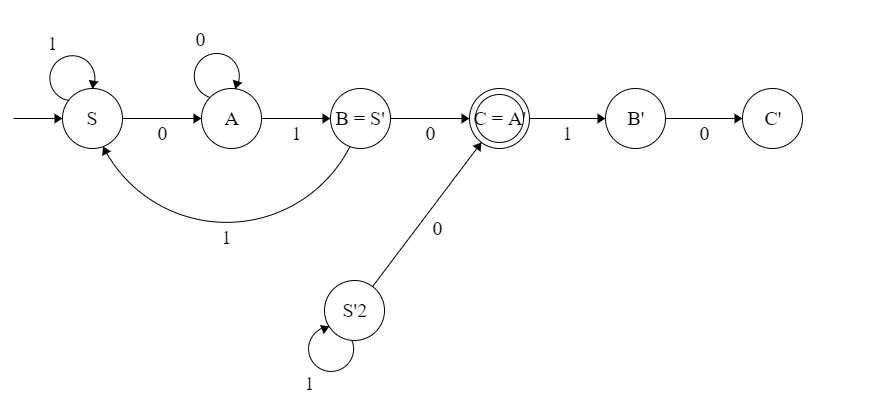
\includegraphics[width=\linewidth]{./exams/misc/02/step_3.png}
\end{center}

Whenever in the later parts we would move back to $S'$, instead we will use $S'_2$ so that will correctly loop with the $1$'s instead of throwing us back at the very beginning.

Now I can add the $0$ loop to $C = A'$:

\begin{center}
    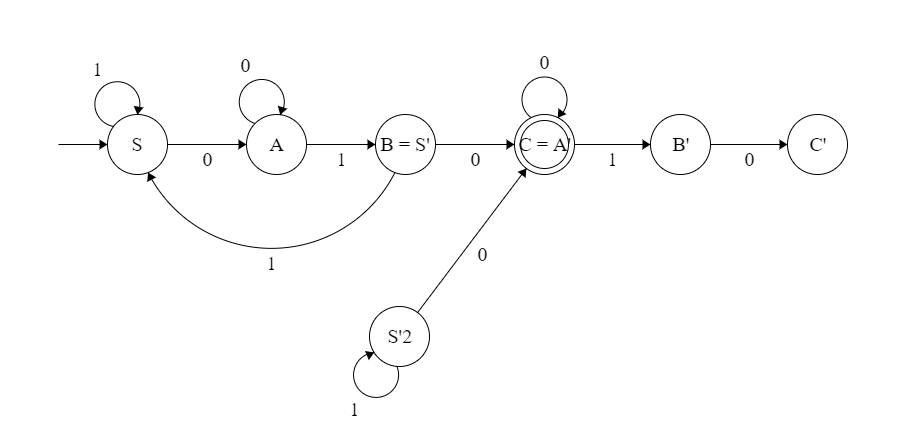
\includegraphics[width=\linewidth]{./exams/misc/02/step_4.png}
\end{center}

Then in $B'$, if we read a $1$ we move back to $S$, and in this case we are going to use our $S'_2$ state, so it cannot escape back to $S$, which we cannot allow:

\begin{center}
    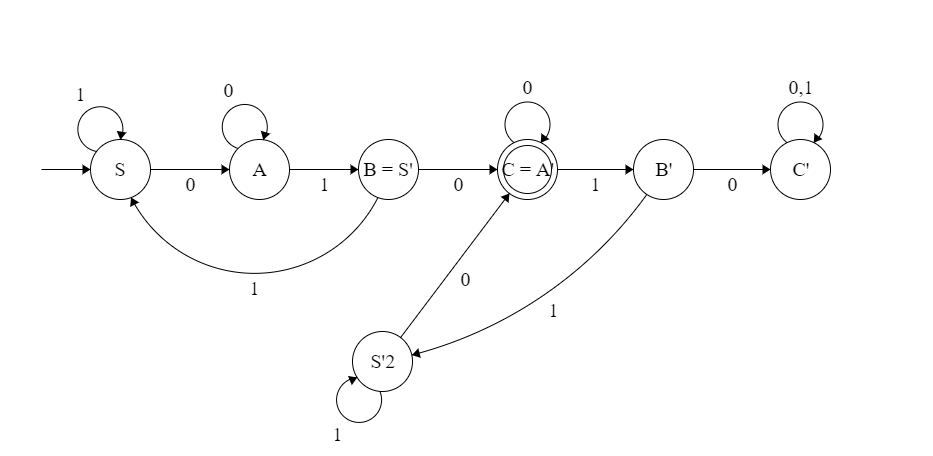
\includegraphics[width=\linewidth]{./exams/misc/02/step_5.png}
\end{center}

And finally I added the $0,1$ loop to $C'$ too, since there we can wait forever.

The new accepting states will be anything new that is not $C'$, since $C'$ means we have found the second $010$ in our input, for which we should fail.

So the final DFA is:

\begin{center}
    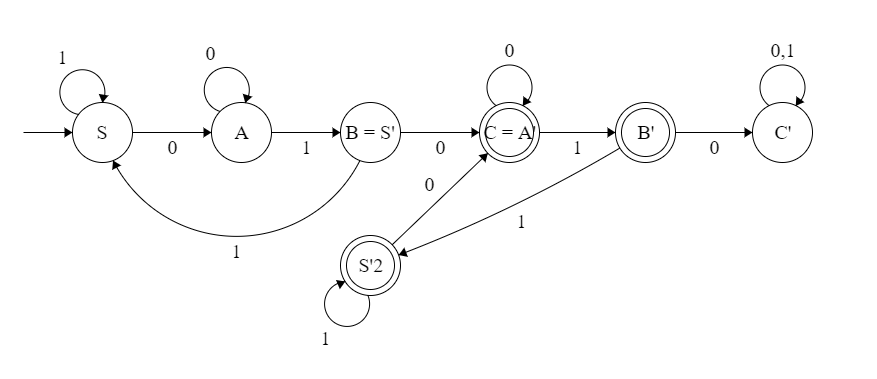
\includegraphics[width=\linewidth]{./exams/misc/02/step_6.png}
\end{center}

So essentially the second $010$ recognizer here is $S'_2, A', B', C'$, and we arrive into it by connecting the last state of the first recognizer, $C$, to the $A'$ state, since we already have the first $0$ when we arrive.